\chapter{Моделирование процессов хемотаксиса бактерий}\label{ch:ch2}

\section{Моделирование процесса генерации степенных распределений на основе механизма дискретного белкового шума}\label{sec:ch2/sec1}
Внутриклеточные сигнальные пути формируют сеть для управления движением бактерии с использованием информации о градиенте концентрации веществ во внеклеточном пространстве. Сеть сигнальных путей процесса хемотаксиса у бактерий E.~coli состоит из небольшого числа компонент, однако этого оказывается достаточно для проявления некоторых свойств сложных биосистем, таких как адаптация и ответ на внешний стимул \cite{korobkova_molecular_2004}. В своей работе авторы показали, что шум, создаваемый сигнальными сетевыми взаимодействиями, контролирует поведенческую вариабельность. Этот механизм демонстрирует свойство биологической системы адаптироваться за счет контроля молекулярного шума. 

Сигнальная сеть хемотаксиса начинается с процесса связывания молекул хемоаттрактанта с сайтами хеморецепторов на цитоплазматической мембране бактерии. Далее, каскад внутриклеточной сигнализации управляет производством белка CheY-P, который диффундирует к моторам и модулирует переключение направления вращения. Изменение направления вращения жгутиков по часовой стрелке (CW) на вращение против часовой стрелки (CCW) заставляет бактерии менять свой паттерн движения: с вращения на одном месте к прямолинейному движению.

Значительный прогресс в понимании статистики переключения двигателей был достигнут с помощью минимальной модели, учитывающей переходы между двумя состояниями через энергетический барьер \cite{tu_how_2005}. Регулирующий путь сводился к действию фосфорилированной формы сигнальной молекулы CheY-P, так что более высокая концентрация CheY-P приводила к более высокой вероятности перехода CCW в CW \cite{khan_steady-state_1980}. В этой работе было обнаружено, что гауссовский шум с конечным временем корреляции может приводить к масштабированию распределений длительностей вращения моторов против часовой стрелки. Подобные флуктуации может вызывать внутренняя стохастичность сигнального генетического пути, в частности, <<генетический шум>> связанный с конечным числом реагирующих белковых молекул.

Для демонстрации возможности возникновения переключений с промежуточной степенной статистикой в связи с генетическим шумом в данном разделе рассматривается модель химической кинетики синтеза белка CheY-P и возникающего в результате переключения вращения моторов. 

Рассмотрим минимальную модель сигнального пути с точки зрения химической кинетики. Переходы между различными значениями числа молекул белка CheY-P, обозначенного $Y$, задаются следующим уравнением:
\begin{equation}
    \begin{aligned}
        Y \mathrel{\mathop{\rightleftarrows}^{\mathrm{K_{y}^{+}}}_{\mathrm{K_{y}^{-}}}} Y + 1,
    \label{eq:chem}
    \end{aligned}
\end{equation}
где $K_{y}^{+}=\frac{Y_0}{\tau}$, $K_{y}^{-}=\frac{Y+1}{\tau}$ -- коэффициенты интенсивностей перехода между состояниями, $Y_0$ -- равновесное число молекул, $\tau$ -- характерное время релаксации сигнального пути к равновесному числу молекул. Являясь элементарным процессом рождения-смерти, по своей сути содержит все необходимые свойства: стохастичность, дискретность состояний и конечное время корреляции $\tau$. Значение $Y_0$ можно принять постоянным в связи с тем, что концентрация хемоаттрактанта изменяется медленно (в процессе движения клетки в слабом градиенте или при изменении уровня хемоаттрактанта во времени) по сравнению со шкалой времени переключения. 

По аналогии рассмотрим модель переключения вращения жгутиков. Пусть $X = 0$ соответствует режиму вращения по часовой стрелке, а $X = 1$ — против часовой стрелки:
\begin{equation}
    \begin{aligned}
        X \mathrel{\mathop{\rightleftarrows}^{\mathrm{K_{x}^{+}}}_{\mathrm{K_{x}^{-}}}} X + 1
    \label{eq:turning}
    \end{aligned}
\end{equation}
где коэффициенты $K_x^{+}=K^{+}(1-X)$, $K_x^{-}=K^{-}X$ ограничивают состояния $X={0, 1}$ и переходы контролируются состоянием регулирующего белка CheY-P через соответствующие интенсивности переключения:
\begin{equation}
    \begin{aligned}
        K^{\pm}=K_0 \exp(\pm\alpha^\pm \cdot \frac{Y_0-Y}{Y_0})
    \label{eq:turning-rates}
    \end{aligned}
\end{equation}
где $\alpha^\pm>0$ характеризует чувствительности интенсивностей переходов, при этом энергетические барьеры аппроксимируются линейной зависимостью относительно уровня CheY-P \cite{khan_steady-state_1980}.

Опишем качественное поведение предложенной модели. Пусть жгутики вращаются по часовой стрелке, что соответствует вращению бактерии на одном месте: $X=0$, а интенсивности соответственно равны $K_x^{+}=K^{+}$ и $K_x^{-}=0$. При уровне белка CheY-P ниже равновесного состояния $Y<Y_0$ интенсивность (частоту) переключения в сторону вращения жгутиков против часовой стрелки (то есть прямолинейного движения бактерии) доминирует: $K^{+}>K_0$. Большие значения уровня белка CheY-P $Y>Y_0$, наоборот уменьшает интенсивность (частоту) переключений. Соответственно при вращении жгутиков против часовой стрелки смещение уровня белка выше или ниже равновесного состояния приводит к обратному эффекту. Отличающиеся друг от друга уровни интенсивности в свою очередь позволяют независимо настраивать интенсивности переходов между движение бактерии вперед и вращением на месте.

Однако в рассмотренной модели есть недостаток: интенсивности переходов могут принимать значения экспоненциально большие или экспоненциально малые в ответ на изменение концентрации $Y$, что может быть биологически неправдоподобным. В соответствии с работой \cite{frankel_adaptability_2014} для учета конечного числа связываний белков CheY-P с моторами, интенсивности переходов могут быть заменены на:
\begin{equation}
    \begin{aligned}
        K^{\pm}=K_0^{\pm} \exp \left (\pm\frac{\alpha^\pm}{2} \left (\frac{1}{2} - \frac{Y}{Y+K_d} \right ) \right )
    \label{eq:turning-rates-kd}
    \end{aligned}
\end{equation}
Такие коэффициенты соответствуют насыщению с уровнем числа белков, превышающем константу диссоциации $K_d$.

Исследование статистических свойств модели было выполнено с помощью численного моделирования уравнений \cref{eq:chem,eq:turning,eq:turning-rates,eq:turning-rates-kd} с применением стохастического алгоритма Гиллеспи \cite{gillespie_stochastic_2007}. В результате численных расчетов был получен набор реализаций, состоящих из $N=10^7$ шагов, соответствующих одной из возможных химических реакций. Один из типов реакции это переключение направления вращения моторов (уравнение \cref{eq:turning}). Непрерывные участки времени пребывания в каждом состоянии CW и CCW соответственно (между переключениями моторов) обозначим $\{t_{ccw}\}$ и $\{t_{cw}\}$. Всего было собрано не менее $N_{cw} = N_{ccw} = 10^{10}$ отрезков времени пребывания в состояниях CW и CCW.

Полученные выборки были использованы для оценки функций плотности вероятности $p(t_{cw})$ и $p(t_{ccw})$ и проанализированы зависимости от времени релаксации сигнального пути $\tau$ и чувствительности интенсивностей переходов между состояниями $\alpha^{\pm}$. Полученные функции плотности вероятности были аппроксимированы степенной функцией на отрезке $[a, b]$ с использованием линейной регрессии в двойном логарифмическом масштабе методом наименьших квадратов. Качество аппроксимации оценивалось коэффициентом детерминации \cite{magnus_2021}, $R^2 \in [0, 1]$. Отрезок $[a, b]$ выбирался перебором с условиями: длина отрезка не менее $1.3$ декады и коэффициент детерминации $R^2 > 0.98$. Если такой отрезок не был найден, то гипотеза об участке со степенным распределением отвергается. 

Рассмотрим простую форму интенсивностей, заданной уравнением \cref{eq:turning-rates}, и оценим плотности вероятности длительностей для соответственно двух состояний CW (вращение бактерии на одном месте) и CCW (прямолинейное движение). В случае отсутствия молекул CheY-P, $Y=0$ (переключение нечувствительно к CheY-P, $\alpha_{\pm}=0$), процесс является пуассоновским, а плотности вероятности длительностей пребывания в состояниях экспоненциальны, $p(t_{ccw}), p(t_{cw}) \propto \exp(-K_0 t)$.

Далее проводился численный анализ для случая равных чувствительностей переключения $\alpha_\pm = \alpha$. Численные результаты показывают, что коррелированный молекулярный шум дает степенное распределение длительностей, $p(t_{ccw}) \approx t^{-\gamma}$, в четко выраженном интервале (1.5-2 декады) с отсечкой при больших значениях длительности. (Рис. \cref{fig:duration-pdf}а).
Плотности с промежуточной степенной асимптотикой на более чем 2 декадах и затухающей с почти экспоненциальной отсечкой, типичны как для измерений in vivo и in vitro пространственной активности бактерий \cite{korobkova_molecular_2004,harris_generalized_2012}.

\begin{figure}[ht]
    \begin{minipage}[b][][b]{0.49\linewidth}\centering
        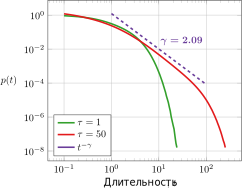
\includegraphics[width=1\linewidth]{genetic-noise/ru/fig1a} \\ (а)
    \end{minipage}
    \hfill
    \begin{minipage}[b][][b]{0.49\linewidth}\centering
        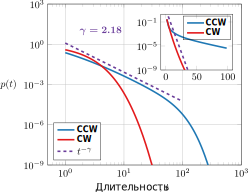
\includegraphics[width=1\linewidth]{genetic-noise/ru/fig1b} \\ (б)
    \end{minipage}
    \caption{
        (а) Плотности вероятности длительностей в состоянии CCW для различных значений времени релаксации белка CheY-P, $\tau$. Остальные параметры: $\alpha = 10$, $Y_0 = 20$, $K_0 = 1$; (б) Плотности вероятности длительностей CW и CCW для $\alpha^+ = 1$, $\alpha^- = 10$, $Y_0 = 20$, $\tau = 50$, $K_0 = 1$. Штриховыми линиями обозначены участки со степенной асимптотикой с показателями $\gamma = 2.09$ (а) и $2.18$ (б), коэффициент детерминации которого $R^2 = 0.98$, количество реализаций $N_{ccw} = N_{cw} = 10^{10}$, $t \in [1, 100]$. На вставке повторно представлены плотности вероятностей длительностей с логарифмической шкалой по оси ординат.
    }
    \label{fig:duration-pdf}
\end{figure}


В работе \cite{tu_how_2005} аналогично было показано, что уменьшение времени корреляции изменяет это распределение в сторону экспоненциального. Рассмотренная модель также способна воспроизводить экспоненциальную статистику длительности CW одновременно со степенным распределением длительностей CCW. При этом, распределения различны из-за несовпадающих чувствительностей интенсивностей переходов между состояниями, то есть $\alpha_+ \neq \alpha_-$. Поскольку время пребывания в состоянии определяется интенсивностью (частотой) покидания этого состояния, то снижение чувствительности перехода из CW в CCW к уровню белка CheY-P должно приводить к экспоненциальному распределению длительностей CW подобно предельному случаю $\alpha^+ = 0$. На рисунке \cref{fig:duration-pdf}б продемонстрирован пример данного режима системы.

Численное моделирование в широком диапазоне параметров показывает, что степенные распределения возникают только тогда, когда время релаксации уровня CheY-P существенно больше, чем время переключения между состояниями CW и CCW $\tau \gg \frac{1}{K_0}$ (Рис. \cref{fig:pdf-gamma-grid-1}а,б). В то же время, увеличение среднего числа сигнальных молекул $Y_0$, приводит к отклонению гипотезы о степенном распределении (Рис. \cref{fig:pdf-gamma-grid-1}а,б). Увеличение числа сигнальных молекул приводит к относительному уменьшению флуктуаций, что в свою очередь уменьшает влияние генетического шума. Параметр чувствительности $\alpha$ контролирует переход между степенным и экспоненциальным распределением длительностей (Рис. \cref{fig:pdf-gamma-grid-1}а). Значения показателя степени $\gamma$, найденные в большей части области параметров ($1 < \gamma < 3$) согласуются с экспериментальными наблюдениями, которые оценили степенной показатель для кумулятивного распределения длительностей CCW как $\gamma - 1 \approx 1.5$. Это свидетельствуют о том, что медленное метилирование как часть сигнального пути отвечает за длительные временные корреляции в выходном сигнале, что приводит к степенному распределению длительностей \cite{korobkova_molecular_2004}. 


\begin{figure}[ht]
    \begin{minipage}[b][][b]{0.49\linewidth}\centering
        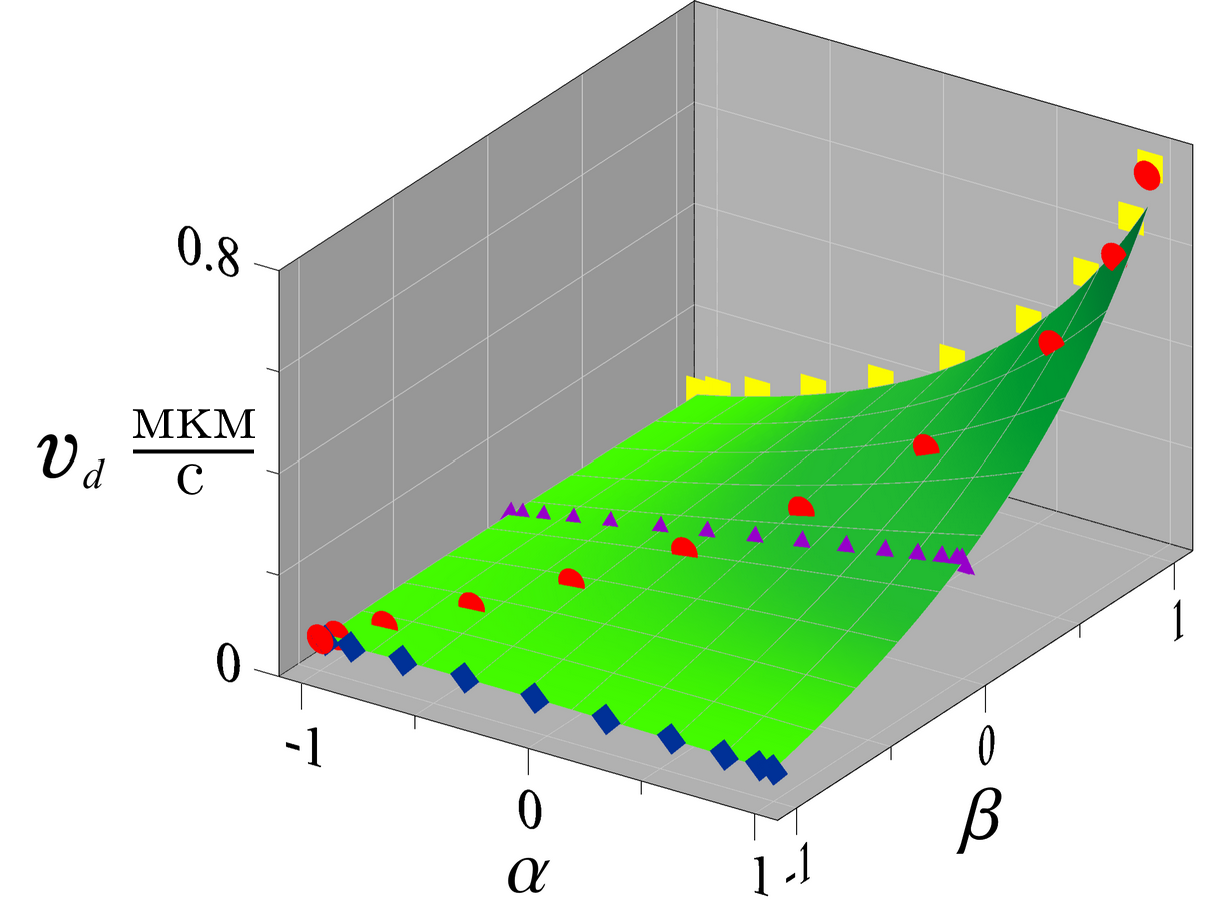
\includegraphics[width=1\linewidth]{genetic-noise/ru/fig2a} \\ (а)
    \end{minipage}
    \hfill
    \begin{minipage}[b][][b]{0.49\linewidth}\centering
        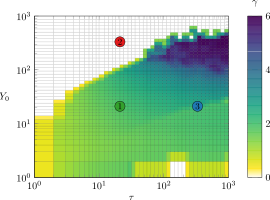
\includegraphics[width=1\linewidth]{genetic-noise/ru/fig2c} \\ (б)
    \end{minipage}\\
    \begin{minipage}[b][][b]{0.49\linewidth}\centering
        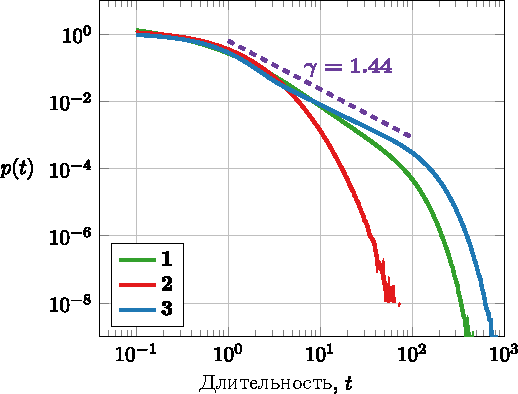
\includegraphics[width=1\linewidth]{genetic-noise/ru/fig2b} \\ (в)
    \end{minipage}
    \hfill
    \begin{minipage}[b][][b]{0.49\linewidth}\centering
        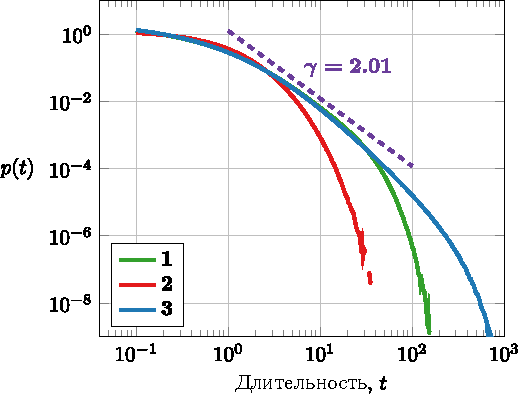
\includegraphics[width=1\linewidth]{genetic-noise/ru/fig2d} \\ (г)
    \end{minipage}
    \caption{
        Показатель степени $\gamma$ для степенного участка плотности вероятности длительности CCW в зависимости от двух параметров: (a) среднего числа молекул CheY-P $Y_0$ и чувствительности $\alpha$ для фиксированного $\tau = 50$, (б) среднего числа молекул CheY-P $Y_0$ и времени корреляции $\tau$ при фиксированных $\alpha = 10$ и $K_0 = 1$. В белой области не наблюдается степенная асимптотика распределений длительности (гипотеза о наличии степенного участка отклоняется). Плотности для комбинаций параметров, отмеченных на панелях (а) и (б) цифрами 1,2,3, показаны на панелях (в) и (г) соответственно. 
    }\label{fig:pdf-gamma-grid-1}
\end{figure}

Далее рассмотрим более приемлемую с биологической точки зрения модель скорости перехода в соответствии с уравнением \cref{eq:turning-rates-kd}, которая имеет насыщение в интенсивностях переключения моторов. Для демонстрации крайних случаев эффекта насыщения рассмотрим ситуацию, когда уровень белка CheY-P находится на равновесном уровне $Y = Y_0$ и константа диссоциации меньше значения уровня равновесия $K_d < Y_0$. Результаты численного моделирования данной модели аналогично подтверждают, что медленная релаксация белка CheY-P вместе с более высокой чувствительностью интенсивности перехода от CCW к CW к изменению уровня белка приводят к появлению степенной асимптотики длительностей CCW, в то время как длительности CW остаются экспоненциально распределенными (Рис. \cref{fig:pdf-kd-powerlaw}).

\begin{figure}[ht]
    \centering
    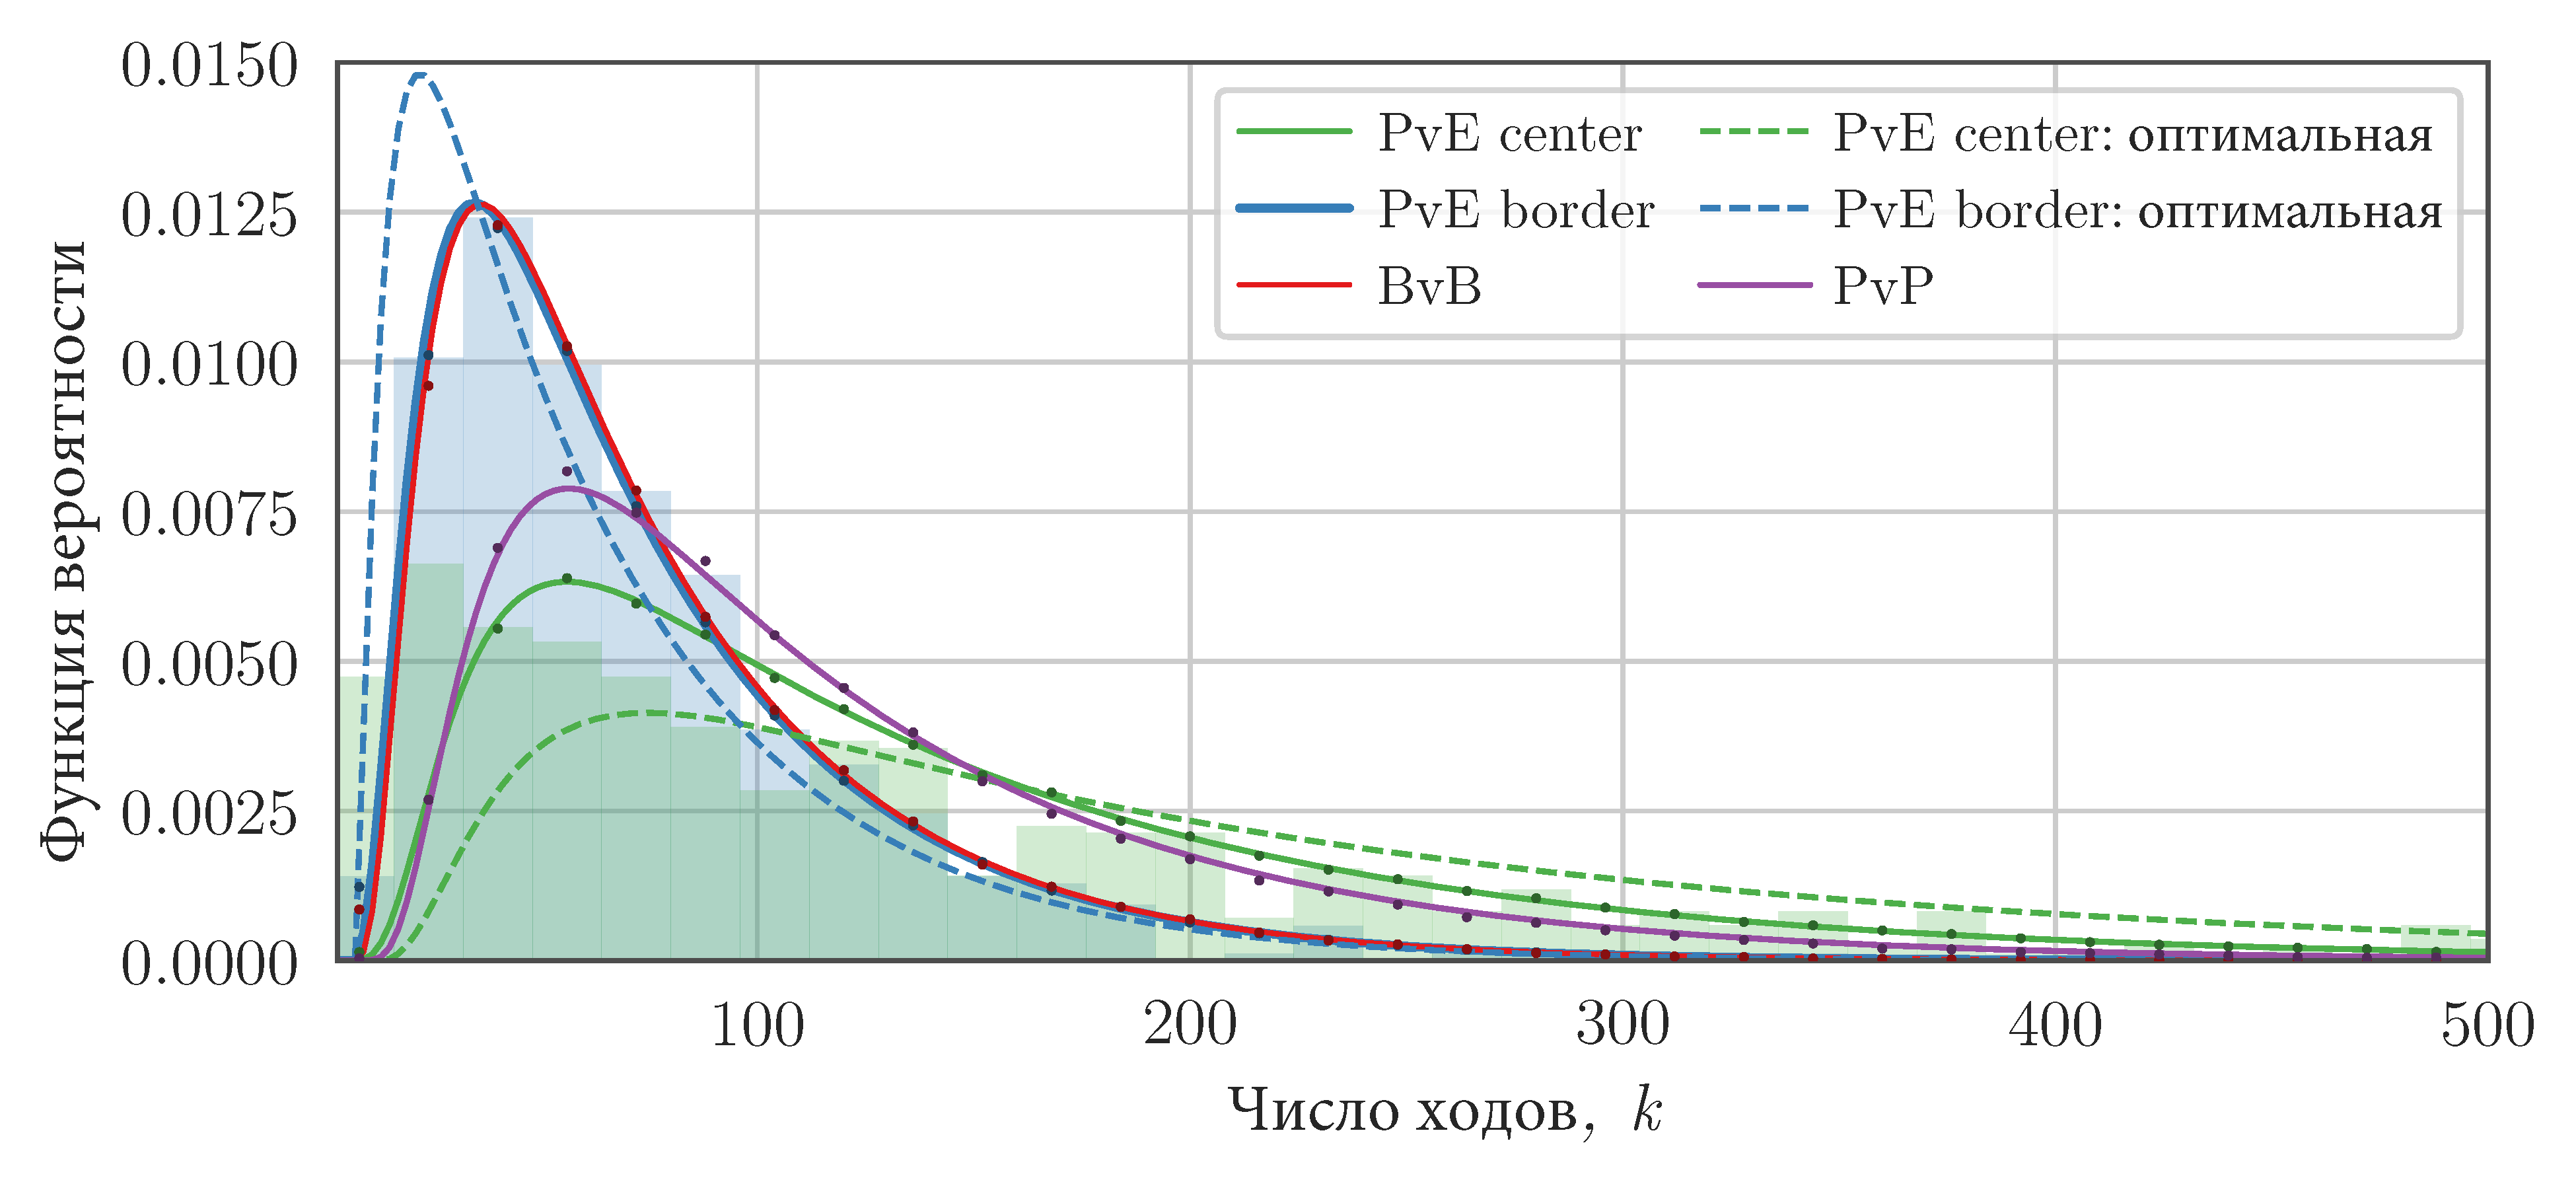
\includegraphics[width=0.5\linewidth]{genetic-noise/ru/fig3}
    \caption{
        Плотность вероятности длительности для состояний CW и CCW при $\alpha^- = 30$, $\alpha^+ = 1$, $Y_0 = 10$, $\tau = 50$, $K_d = 2$, $K^+_0 = 100$, $K^-_0 = 0.2$. Штриховая линия -- степенная зависимость с $\gamma = 3.18$, $R^2 = 0.999$, $N_{ccw} = 10^{11}$, $t \in [0.1, 20]$. На вставке повторно представлены плотности вероятностей длительностей с логарифмической шкалой по оси ординат.
    }
    \label{fig:pdf-kd-powerlaw}
\end{figure}



Систематическое исследование статистики в зависимости от значений параметров модели представлено на Рис. \cref{fig:pdf-gamma-grid-kd}. На плоскости параметров $(K_d, Y_0)$ выделяются две области, соответствующие двум различным вариантам поведения модели (Рис. \cref{fig:pdf-gamma-grid-kd}а). При $Y_0 < K_d$ эффект насыщения имеет слабое влияние, что приводит к сильному отклонению от степенной асимптотики по мере увеличения константы диссоциации. Степенная асимптотика проявляется при достаточно малых показателях $\gamma < 2$. Для $Y_0 > K_d$ введенный эффект насыщения приводит к большим значения показателя $\gamma > 4$ в степенной асимптотике. 

На другой плоскости параметров $(K_d, \alpha_-)$ степенная асимптотика сохраняется в широком диапазоне параметра чувствительности перехода от CCW к CW, $\alpha_-$ (Рис. \cref{fig:pdf-gamma-grid-kd}б). Аналогично выделяются режимы с относительно малыми $\gamma < 2$ и большими $\gamma > 4$ значениями показателя степени. Эти режимы обусловлены соотношением между средним числом молекул CheY-P, $Y_0$, и насыщением константы диссоциации $K_d$.

\begin{figure}[ht]
    \begin{minipage}[b][][b]{0.49\linewidth}\centering
        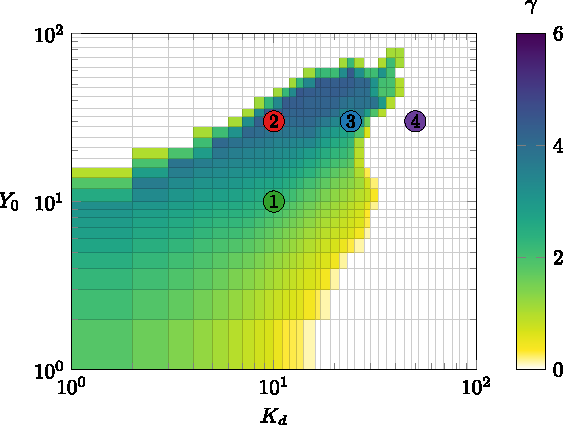
\includegraphics[width=1\linewidth]{genetic-noise/ru/fig4a} \\ (а)
    \end{minipage}
    \hfill
    \begin{minipage}[b][][b]{0.49\linewidth}\centering
        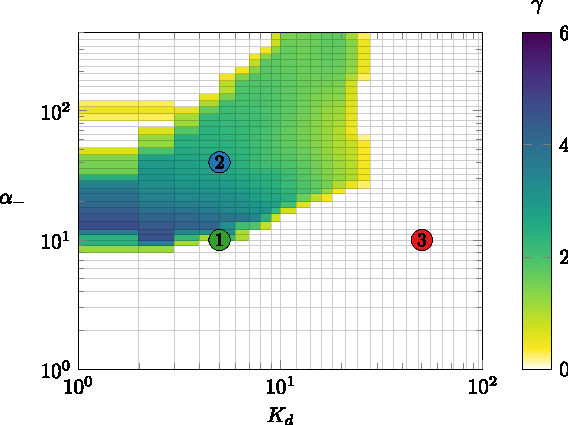
\includegraphics[width=1\linewidth]{genetic-noise/ru/fig4c} \\ (б)
    \end{minipage}\\
    \begin{minipage}[b][][b]{0.49\linewidth}\centering
        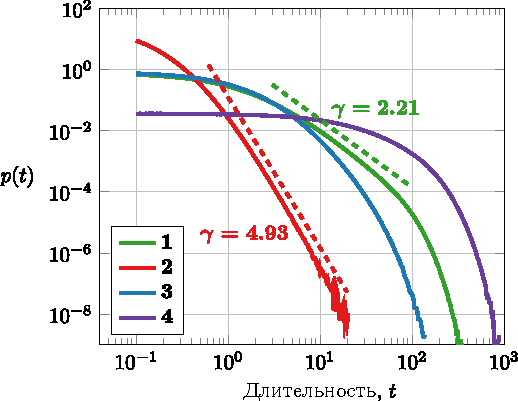
\includegraphics[width=1\linewidth]{genetic-noise/ru/fig4b} \\ (в)
    \end{minipage}
    \hfill
    \begin{minipage}[b][][b]{0.49\linewidth}\centering
        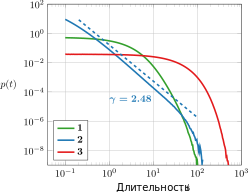
\includegraphics[width=1\linewidth]{genetic-noise/ru/fig4d} \\ (г)
    \end{minipage}
    \caption{
        Показатель степени $\gamma$ для степенного участка плотности вероятности длительности CCW в зависимости от двух параметров: (a) константы насыщения $K_d$ и среднего числа молекул CheY-P $Y_0$ для фиксированного параметра $\alpha^- = 30$, (б) константы насыщения $K_d$ и параметра чувствительности $\alpha^-$ при фиксированном параметре $Y_0 = 10$. Остальные параметры модели были выбраны $\alpha^+=1$, $\tau=50$, $K^+_0=100$, $K^-_0=0.2$. В белой области не наблюдается степенная асимптотика распределений длительности (гипотеза о наличии степенного участка отклоняется). Плотности для комбинаций параметров, отмеченных на панелях (а) и (б) цифрами 1,2,3,4, показаны на панелях (в) и (г) соответственно. 
    }\label{fig:pdf-gamma-grid-kd}
\end{figure}


Таким образом биологически релевантная модель дает наиболее схожие с экспериментом показатели степени при коэффициенте диссоциации близком к константе диссоциации $K_d \approx Y_0$ при этом со значениями не превышающими $30$ молекул. Управление параметром $\alpha_-$ в свою очередь позволяет получить степенную асимптотику на большем числе декад, сохранив ее также на меньших промежутках длительностей нахождения в состоянии CCW.

Хотя применение подхода численного моделирования с применением алгоритма Гиллеспи обладает гибкостью к нахождению численных решений произвольных задач, временные затраты на вычисление ограничивают возможности применения модели. Подход full-counting statistics, впервые предложенный в работах по квантовой физике \cite{levitov_electron_1996}, позволяет независимо от природы основного кинетического уравнения оценить статистические свойства дискретной системы. Далее рассмотрим как данный подход может быть использован для вычисления статистики переключения моторов напрямую из интенсивностей перехода $K_x^\pm(Y)$ и $K_y^\pm(Y)$.

Рассмотрим кинетику модели, заданной уравнениями \cref{eq:chem,eq:turning}, в терминах марковских процессов с непрерывным временем \cite{tikhonov_markov_process_1977}. Диаграмма переходов представлены на рис. \cref{fig:transitions}. Состояние $Z(t)$ процесса в момент времени $t$ представляет собой двумерный вектор $Z = (X, Y)$, где первая компонента представляет направление вращения моторов $X = 0 \equiv \mathrm{CW}$ (по часовой стрелке) и $X = 1 \equiv \mathrm{CCW}$ (против часовой стрелки), а вторая компонента $Y$ -- количество молекул CheY-P. Тогда основное кинетическое уравнение для вектора вероятности $\mathrm{P}(Z, t) \equiv \mathrm{P}(X, Y, t)$ имеет вид:

\begin{equation}
    \begin{aligned}
        &\dot{\mathrm{P}}(\mathrm{CW},0,t)&=&-\left (\frac{Y_0}{\tau} + K_x^+(0) \right ) \mathrm{P}(\mathrm{CW},0,t) + K_x^-(0) \mathrm{P}(\mathrm{CCW},0,t)+&&\\
        &&&+\frac{1}{\tau}\mathrm{P}(\mathrm{CW},1,t),&&\\
        &\dot{\mathrm{P}}(\mathrm{CCW},0,t)&=&-\left (\frac{Y_0}{\tau} + K_x^-(0) \right ) \mathrm{P}(\mathrm{CCW},0,t) + K_x^+(0) \mathrm{P}(\mathrm{CW},0,t)&&\\
        &&&+\frac{1}{\tau}\mathrm{P}(\mathrm{CCW},1,t),&&\\
        &\dots&&\\
        &\dot{\mathrm{P}}(\mathrm{CW},Y,t)&=&-\left (\frac{Y_0+Y}{\tau} + K_x^+(Y) \right ) \mathrm{P}(\mathrm{CW},Y,t) + K_x^-(Y) \mathrm{P}(\mathrm{CCW},Y,t)+&&\\
        &&&+\frac{Y+1}{\tau}\mathrm{P}(\mathrm{CW},Y+1,t)+\frac{Y_0}{\tau}\mathrm{P}(\mathrm{CW},Y-1,t),&&\\
        &\dot{\mathrm{P}}(\mathrm{CCW},Y,t)&=&-\left (\frac{Y_0+Y}{\tau} + K_x^-(Y) \right ) \mathrm{P}(\mathrm{CCW},Y,t) + K_x^+(Y) \mathrm{P}(\mathrm{CW},Y,t)+&&\\
        &&&+\frac{Y+1}{\tau}\mathrm{P}(\mathrm{CCW},Y+1,t)+\frac{Y_0}{\tau}\mathrm{P}(\mathrm{CCW},Y-1,t).&&\\
    \end{aligned}
    \label{eq:master-transitions}
\end{equation}


\begin{figure}[ht]
    \centering
    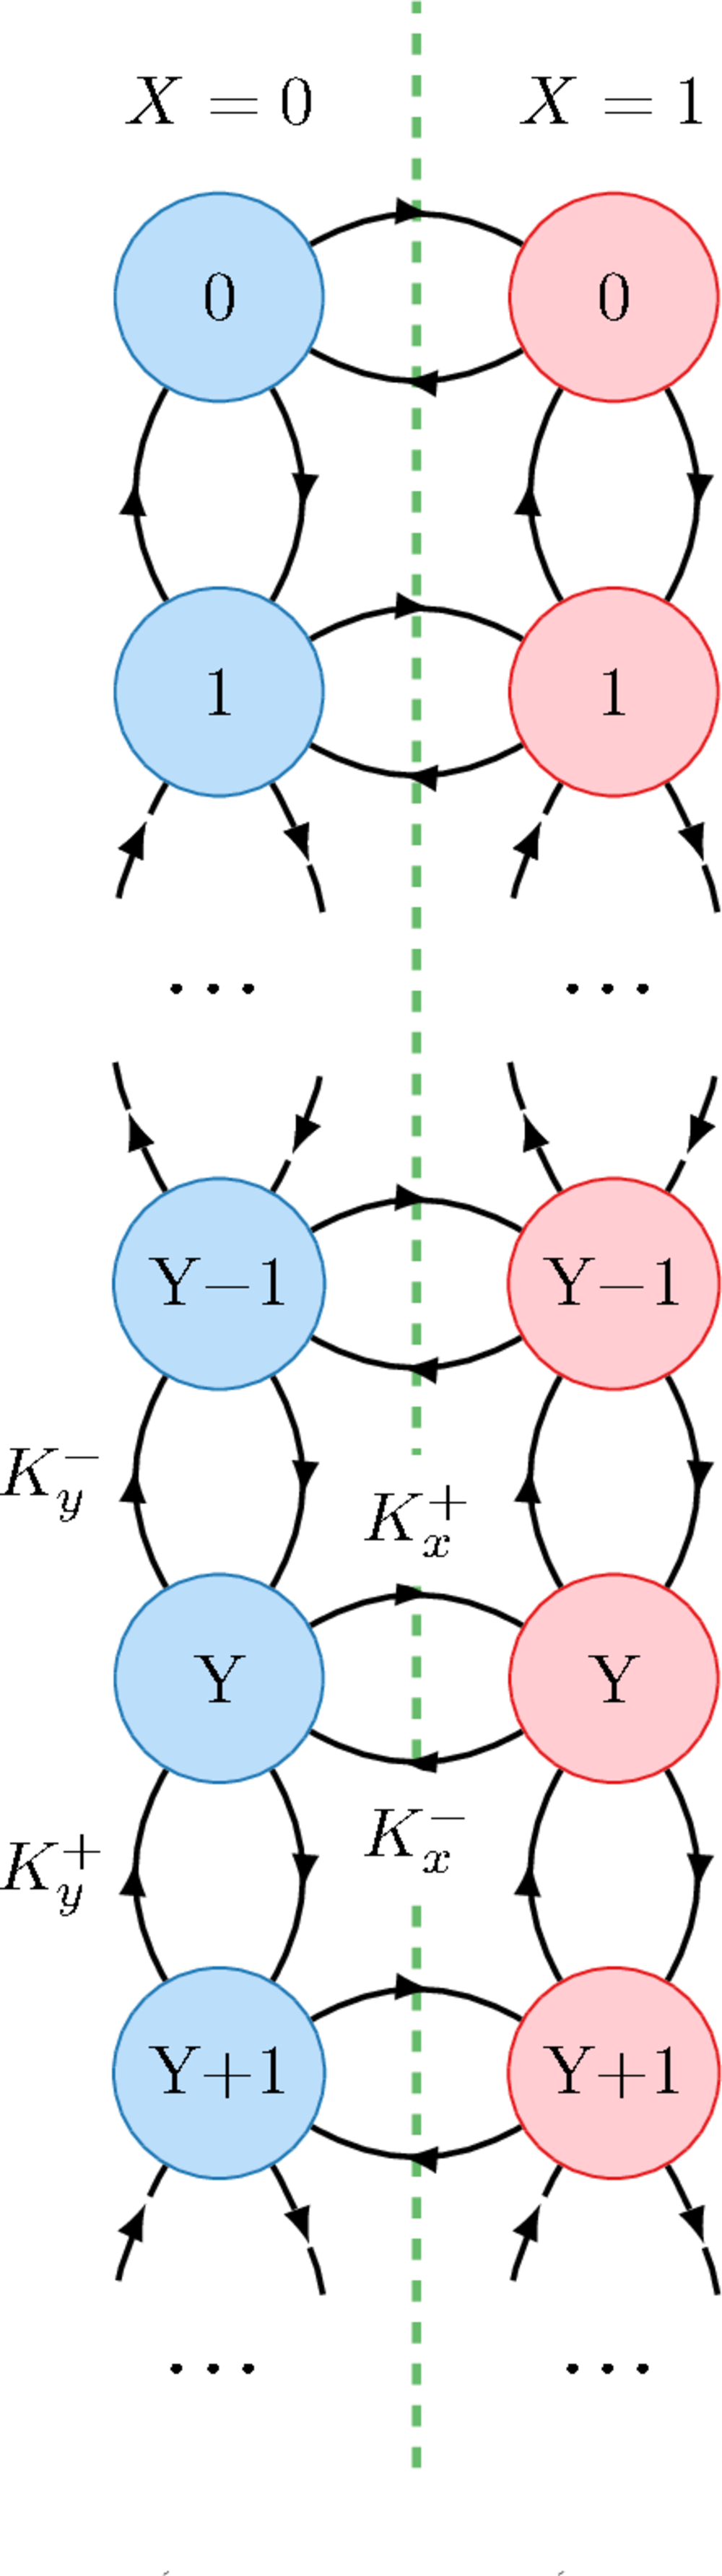
\includegraphics[width=0.25\linewidth]{genetic-noise/ru/fig0}
    \caption{
        Диаграмма переходов марковского процесса \cref{eq:master-transitions}, построенного для кинетической модели, описываемой уравнениями \cref{eq:chem,eq:turning}.
    }
    \label{fig:transitions}
\end{figure}

Примечательно, что наша модель служит обобщением жидкостной очереди, управляемой процессом рождения-смерти, предложенным ван Доорном, Ягерсом и де Витом \cite{van_doom_fluid_1988}. В терминах марковских процессов реакция \cref{eq:turning} представляет собой обмен вероятностью между двумя состояниями. Этот обмен можно рассматривать как обмен фиксированного количества несжимаемой жидкости между двумя баками со скоростями, определяемыми состоянием процесса рождения-смерти. В исходной постановке задачи был только один бак бесконечного объема и неограниченное количество жидкости. Длительность в состоянии CCW -- это время, которое одна молекула жидкости проводит в резервуаре <<1>>, прежде чем покинуть его. Введем вектор вероятности нахождения в каждом состоянии марковской цепи: 

\begin{equation}
    P(t) = \begin{bmatrix}
    P(X = \mathrm{CW}, Y = 0; t)\\
    P(X = \mathrm{CW}, Y = 1; t)\\
    P(X = \mathrm{CW}, Y = 2; t)\\
    ...\\
    P(X = \mathrm{CCW}, Y = 0; t)\\
    P(X = \mathrm{CCW}, Y = 1; t)\\
    P(X = \mathrm{CCW}, Y = 2; t)\\
    ...\\
    \end{bmatrix}
\label{eq:state-probs}
\end{equation}

Также для марковской цепи определим матрицу интенсивностей переходов $\boldsymbol{\mathrm{Q}}$ \cite{kapmen_stochastic_1990}. Тогда уравнение \cref{eq:master-transitions} представляется в компактной форме: 

\begin{equation}
    \boldsymbol{\mathrm{P}}(t) = \boldsymbol{\mathrm{Q}} \boldsymbol{\mathrm{P}}(t),
    \label{eq:master-transitions-compact}
\end{equation}
где матрица $\boldsymbol{\mathrm{Q}}$ состоит из суммы двух матриц: матрицы интенсивностей переходов процесса рождения-гибели для числа молекул, состоящей из двух одинаковых полубесконечных трехдиагональных блоков $\boldsymbol{\mathrm{Q}}_{BD}$; и матрицы, определяющей интенсивности переходов между сменой направления вращения моторов, состоящей из диагональных блоков:

\begin{equation}
    \boldsymbol{\mathrm{Q}}_{R} = 
    \begin{bmatrix} \mathrm{diag}\{-K^+_x (Y)\}&\mathrm{diag}\{+K^-_x (Y)\}\\ \mathrm{diag}\{+K^+_x (Y)\}&\mathrm{diag}\{-K^-_x (Y) \} \end{bmatrix},
    \label{eq:transition-block}
\end{equation}
где $\mathrm{diag}\{x_k\}$ -- обозначение полубесконечного диагонального матричного блока с элементами $x_k$ на диагонали.

Далее рассмотрим вероятность $P_A(t)$ отсутствия перехода из состояния CCW в состояние CW в течение времени $t$. Для этого определим вектор начального распределения по состояниям $(\mathrm{CCW}, Y)$:

\begin{equation}
    \boldsymbol{\mathrm{P_S}} = 
    \begin{bmatrix} P(\mathrm{CCW}, Y, 0)\\ \end{bmatrix}_Y.
    \label{eq:start-prob}
\end{equation}

Для выбранного начального состояния, вероятность $P_A(t)$ может быть вычислена на основе вектора условных вероятностей обнаружения молекулы в момент времени $t$ в состоянии $(\mathrm{CCW}, Y)$ после $k$ переходов, рассмотренного при $k=0$ \cite{mordovina_full-counting_2013}: 
\begin{equation}
    \boldsymbol{\mathrm{P}}^{(k)}(t) = \begin{bmatrix} \boldsymbol{\mathrm{P}}^{(k)}(\mathrm{CCW}, Y, t)\end{bmatrix}_Y.
    \label{eq:conditioned-transitions}
\end{equation}

Эволюция этого вектора при $k=0$ определяется соответствующим основным кинетическим уравнением:

\begin{equation}
    \dot{\boldsymbol{\mathrm{P}}}^{(0)}(t)=\boldsymbol{\mathrm{Q}}_{NT}\mathrm{P}^{(0)}(t) = \left (\boldsymbol{\mathrm{Q}}_{BD} - \boldsymbol{\mathrm{Q}}_{10} \right ),
    \label{eq:conditioned-master-transtions}
\end{equation}
где $\boldsymbol{\mathrm{Q}}_{10} = \mathrm{diag}\{-K^-_x(Y)\}$ -- диагональная матрица с интенсивностями переходов из состояния CCW в состояние CW.

Тогда вероятность остаться в состоянии CCW выражается следующей суммой:
\begin{equation}
    P_A(t) = \sum_Y \mathrm{P}^{(0)}(\mathrm{CCW},Y,t).
    \label{eq:no-transition-prob}
\end{equation}

Матрица $\boldsymbol{\mathrm{Q}}_{NT}$ -- полубесконечная трехдиагональная матрица с положительными недиагональными элементами (матрица Якоби). Такая матрица имеет чисто вещественный невырожденный спектр ${\lambda_1, \lambda_2, ..., \lambda_i, ...}$. Наибольшее собственное значение отрицательное, $\lambda_1 < 0$, то есть существует <<утечка вероятности>> из состояния $X = \mathrm{CCW}$ в состояние $X = \mathrm{CW}$, так что основное кинетическое уравнение \cref{eq:master-transitions} не сохраняет норму вектора, и, соответственно, все остальные собственные числа также отрицательные $\lambda_i < 0$. 

Расчет вектора условной вероятности в любой момент времени может быть произведен путем спектрального разложения матрицы $\boldsymbol{\mathrm{Q}}_{NT}$:

\begin{equation}
    \boldsymbol{\mathrm{P}}^{(0)}(t) = \sum_i \alpha_i \exp(\lambda_i t) v_i,
    \label{eq:solution-no-transition-prob}
\end{equation}
где $\alpha_i=w_i^T \boldsymbol{\mathrm{P_S}}$, $\boldsymbol{w_i}$ -- набор левых собственных векторов матрицы $\boldsymbol{\mathrm{Q}}_{NT}$, $\boldsymbol{v_i}$ -- набор правых собственных векторов матрицы $\boldsymbol{\mathrm{Q}}_{NT}$. Затухание $P_A(t)$ с увеличением времени происходит монотонно из-за свойств спектра.

Для вычисления плотности вероятности $p(t)$ длительности нахождения в состоянии CCW, необходимо вычислить $P_A(t)$ для начального вектора $\boldsymbol{\mathrm{P_S}}$, соответствующего распределению по состояниям $Y$ в момент, когда происходит переход из состояния CW в состояние CCW.
Тогда плотность вероятности записывается следующим образом:

\begin{equation}
    p(t) = -\dot{P_A}(t) = \sum_Y \sum_i -\lambda_i \alpha_i \exp(\lambda_i t) (\boldsymbol{v_i})_Y.
    \label{eq:solution-no-transition-pdf}
\end{equation}

Для получения начального распределения, в момент перехода из состояния CW в состояние CCW, необходимо найти стационарное распределения $\boldsymbol{\mathrm{P_{st}}}$ полной марковской цепи:

\begin{equation}
    \boldsymbol{\mathrm{Q}} \boldsymbol{\mathrm{P_{st}}} = \boldsymbol{0},
    \label{eq:transitions-stationary}
\end{equation}
где $\boldsymbol{0}$ -- нулевой полубесконечный вектор.

Подвектор, соответствующий состоянию CW: ${P_{st}(CW, Y)}$, будет определять вероятность нахождения системы в состоянии $Y$ при условии ее нахождения в CW. Вероятность перехода системы из $(\mathrm{CW}, Y)$ в $(\mathrm{CCW}, Y)$ пропорциональна интенсивности перехода $K_x^+(Y)$. Однако для системы из бесконечного числа состояний относительная частота перехода в общем случае не определена. В связи с этим осуществим переход к конечному числу состояний, в которых сконцентрирована вероятность нахождения системы. 

\begin{equation}
    P_x^+(Y)=\frac{K_x^+(Y)}{\sum_{Y\in W} K_x^+(Y)},
    \label{eq:cw-to-ccw-prob}
\end{equation}
где $W$ -- конечный набор состояний числа молекул $Y$, в которых сконцентрирована вероятность нахождения системы. Оценка на погрешность вычисленных вероятностей в зависимости от подмножества выбранных состояний при переходе к конечномерной системе дается в теореме о проекции марковской цепи на конечное число состояний \cite{munsky_finite_2006}. Также в работе предлагается алгоритм, который дает возможность определить достаточное число состояний для получения необходимой точности.

Тогда по теореме Байеса вероятность нахождения системы в состоянии $(\mathrm{CCW}, Y)$ при условии, что до этого она была в $(\mathrm{CW}, Y)$:
\begin{equation}
    P_S(Y)=\frac{P_{st}(\mathrm{CW}, Y) P_x^+(Y)}{\sum_{Y\in W} P_{st}(\mathrm{CW}, Y) P_x^+(Y)}.
    \label{eq:start-prob-solution}
\end{equation}

Далее было проведено сравнение результатов расчета плотностей вероятностей длительностей методом Гиллеспи и расчета прямым методом, полученным из теории Марковских цепей и подхода full-counting statistics. Вычисление прямым методом сводится к нахождению собственных чисел и векторов матрицы $\boldsymbol{\mathrm{Q}}_{NT}$ и нахождению стационарного распределения марковской цепи. На рисунке \cref{fig:gillespi-vs-direct}. Рассчитанное таким образом распределение длительностей полностью совпадает с распределением, полученным при расчете статистики по множеству реализаций стохастическим алгоритмом Гиллеспи.

\begin{figure}[ht]
    \centering
    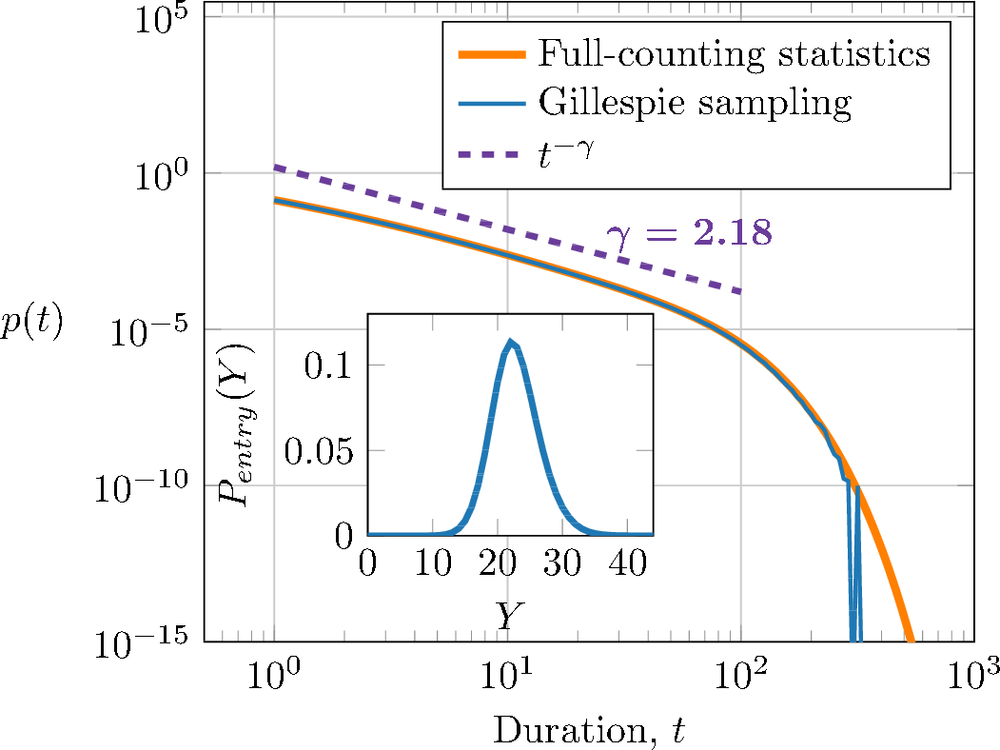
\includegraphics[width=\linewidth]{genetic-noise/ru/fig1c.png}
    \caption{
        Плотности вероятности длительностей CCW, полученные с применением двух подходов: оранжевая линия -- подход full-counting statistics для процесса, описываемого основным уравнением \cref{eq:conditioned-master-transtions}, с усечением при $Y_{max} = 100$; синяя линия -- метод Гиллеспи для исходной кинетической модели \cref{eq:chem,eq:turning}. На вставке показано распределение вероятности $P_S(Y)$ для начального распределения состояний CCW относительно числа молекул $Y$, \cref{eq:start-prob-solution}. Параметры модели были выбраны эквивалентно параметрам на рисунке \cref{fig:duration-pdf}б.
    }
    \label{fig:gillespi-vs-direct}
\end{figure}



\section{Модель движения бактерии с двумя чередующимися событиями поворота}\label{sec:ch2/sec2}

Рассмотренная в предыдущем разделе бактерия E.~coli обладает паттерном движения, состоящим из двух стадий: прямолинейного движения и вращения на одном месте. Однако в зависимости от среды обитания и других факторов эволюционно бактерии выработали различные паттерны движения для ориентации в пространстве. Примером бактерии с характерно другим паттерном служит вид V.~alginolyticus, обитающий в морской среде. Паттерн движения V.~alginolyticus состоит из трех этапов: прямолинейное движение, реверсивное движение и быстрый разворот \cite{xie_bacterial_2011}. В этом паттерне бактерия движется некоторое время вперед, затем направление вращения моторов жгутиков меняются на противоположное и бактерия осуществляет реверсивное движение. При реверсивном движении жгутики бактерии имеют механическую нестабильность, что приводит к третьему этапу разворота бактерии \cite{taute_high-throughput_2015}. Пример движения бактерии реконструированного в эксперименте, приведен на рисунке \cref{fig:vibrio-trajectories}.

Дополнительно было показано, что средний угол разворота зависит от размера клетки, при этом более крупные клетки имеют большие углы разворота \cite{taute_high-throughput_2015}. Это означает, что более крупные клетки стабилизируют движение за счет противодействия силе вязкого сопротивления, действующей на тело клетки, и соответственно угол их поворота получается ближе к реверсивному. 

Далее, применяя формализм де Жена \cite{de_gennes_chemotaxis_2004}, построим модель, описывающую движение бактерии с двумя чередующимися событиями поворота.

Пусть паттерн движения состоит из 4 этапов: 
\begin{enumerate}
  \item <<Вперед-1>>: прямолинейное движение в некотором направлении.
  \item <<$\alpha$-поворот>>: поворот на некоторый случайный угол $\Delta\phi_1$ при котором средний косинус угла равен $\alpha$, то есть $M[\cos (\Delta\phi_1)]=\alpha$.
  \item <<Вперед-2>>: прямолинейное движение в новом направлении.
  \item <<$\beta$-поворот>>: поворот на некоторый случайный угол $\Delta\phi_2$ при котором средний косинус угла равен $\beta$, то есть $M[\cos (\Delta\phi_2)]=\beta$.
\end{enumerate}

Скорость движения бактерии при прямолинейном движении рассматривается как константа, одинаковая для 1 и 3 этапов. Однако, существуют другие виды бактерий, например, P.~putida, обладающие различной скоростью движения чередующихся прямолинейных движений \cite{theves_bacterial_2013}. В данной модели скорости выбраны одинаковыми, чтобы сконцентрироваться на влиянии именно паттерна движения, состоящего из двух различных углов.

Рассматриваемый $\alpha-\beta$ паттерн движения экспериментально наблюдается у различных видов бактерий, таких как P.~haloplanktis, V.~coralliilyticus \cite{son_bacteria_2013}, C.~crescentus \cite{liu_helical_2014}, S.~putrefaciens \cite{stocker_reverse_2011} и других. 

В данном разделе детали модели будем основывать на экспериментальных наблюдениях за бактериями V.~alginolyticus. Экспериментально было продемонстрировано \cite{altindal_implications_2011}, что в отсутствии химического градиента данный вид бактерий демонстрирует среднее время участка прямолинейного движения, одинаковое для первого и третьего этапа паттерна, равное $\tau_{run} \approx 0.3s$. Наблюдаемое в эксперименте распределение длительностей представляет собой экспоненциальное распределение, однако в области коротких времен распределение часто отклоняется от экспоненциального. В рассматриваемой модели будем использовать упрощенное предположение о том, что распределение следует экспоненциальному закону с показателем $\lambda_0=\frac{1}{\tau_{run}}$. Такой выбор связан с упрощением предложенного аналитического анализа. Длительности же второго и четвертого этапов, характеризующих процесс вращения бактерии на одном месте, на порядок меньше, чем длительности прямолинейного движения, в связи с чем ими обычно пренебрегают в моделях \cite{block_adaptation_1983}. В предложенной модели будем рассматривать повороты как мгновенные события.

Движение бактерии сопряжено с тепловым движением жидкости и активными процессами в моторах бактерии, что вызывает отклонения от строго прямолинейного движения. Экспериментально было показано, что такие отклонения согласуются с броуновской вращательной диффузией \cite{berg_chemotaxis_1972}, которая описывается константой $D_r$. Значение константы может быть экспериментально измерено и ее значение согласуется со значением для броуновской вращательной диффузии пассивной частицы с размером характерным для бактерии. Влияние вращательной диффузии может отклонять за этап прямолинейного движения направляющий вектор до $30^\circ$. 

В отсутствии химических веществ траектория для такого паттерна движения представляет собой случайное блуждание, характеризующееся корреляционной функцией скорости и эффективной постоянной долговременной диффузии бактерии, аналитические выражения для которых были найдены в работе Йоханнес Тактикос \cite{taktikos_how_2013}. 

В случае наличия химических веществ в среде, бактерия способна направлять свое случайное блуждание в направлении химического аттрактанта за счет хемосенсорной системы. Работа этой системы обеспечивает интеграцию сигнала во времени и ответную реакцию с некоторой задержкой, изменяющую направление вращения моторов жгутиков. При движении бактерии в направлении градиента длительность этапа прямолинейного движения увеличивается, позволяя бактерии продолжать движение в благоприятную сторону. 

Основной линейной моделью хемотаксиса бактерии является модель де Жена \cite{de_gennes_chemotaxis_2004}, которая связывает частоту переключения направления вращения моторов $\lambda(t)$ со значением концентрации химического вещества $c(t)$, измеренного сенсорами бактерии:

\begin{equation}
    \begin{aligned}
        \lambda(t)=\lambda_0 \left ( 1 - \int_{-\infty}^t R(t-\tau)c(\tau)d\tau \right ),
    \label{eq:turning-frequency}
    \end{aligned}
\end{equation}
где $\lambda_0=\frac{1}{\tau_{run}}$ -- частота переключения в отсутствии химических веществ, $R(t)$ -- внутренняя функция отклика бактерии. В случае с видом бактерий E.~coli функция отклика бактерии была измерена экспериментально в работе \cite{block_adaptation_1983} и аналитически представима в следующем виде:

\begin{equation}
    \begin{aligned}
        R(t) = W \lambda_0 e^{-\lambda_0t} \left ( 1 - \frac{\lambda_0T}{2} - \left (\frac{\lambda_0T}{2}\right )^2 \right )
    \label{eq:response-ecoli}
    \end{aligned}
\end{equation}
где $W$ характеризует силу отклика бактерии.  

Важное свойство функции отклика состоит в способности бактерии подстраиваться под фоновую концентрацию химического вещества и относительно нее распознавать малый градиент. Для учета отсутствия влияния однородной концентрации на частоту функция отклика должны обладать следующим свойством:  
\begin{equation}
    \begin{aligned}
        \int_{-\infty}^{\infty} R(\tau)d\tau = 0
    \label{eq:response-ecoli-zero}
    \end{aligned}
\end{equation}
Тогда в уравнении \cref{eq:turning-frequency} при постоянной концентрации $c(t)\equiv const = c_0$ интеграл также обращается в ноль и $\lambda(t)=\lambda_0$. Таким образом, если функция отклика обладает указанным свойством, то малые изменения $\Delta c(t)$ относительно фоновой концентрации $c_0$ в измеряемой концентрации вещества $c(t)=c_0+\Delta c(t)$ влияют на частоту переключений $\lambda(t)$ независимо от величины $c_0$. 

Ранее в экспериментальных исследованиях была измерена функция отклика для бактерий вида V.alginolyticus \cite{xie_element_2015}, обладающая необходимым свойством. Функции отклика для движения в прямом и реверсивном этапах в общем случае могут различаться \cite{xie_marine_2015}. Далее, для упрощения анализа, предполагается, что функции отклика для обоих вариантов прямолинейного движения совпадают.

Не нарушая общности рассмотрим движение бактерии как случайное блуждание в пространстве, начинающееся с события <<$\alpha$-поворот>> в момент времени $t=0$, затем событие движения <<Вперед-2>> длительностью $t_{\beta}$, соответственно, событие <<$\beta$-поворот>> в момент времени $t=t_{\beta}$ и событие <<Вперед-1>> длительностью $t_{\alpha}$. Определим вектор положения бактерии $\textbf{r}(t)=(x(t),y(t),z(t))$ в момент времени $t$ как сумму смещений $\Delta r_{\alpha}=(\Delta x_{\alpha},\Delta y_{\alpha},\Delta z_{\alpha})$ и $\Delta r_{\beta}=(\Delta x_{\beta},\Delta y_{\beta},\Delta z_{\beta})$ соответствующих парам событий. 

Дополнительно определим функцию плотности вероятности длительностей $t$ участков прямолинейного движения $p(t)=p_{\alpha}(t)=p_{\beta}(t)$. 

Описанная модель будет использована для дальнейшего анализа скорости смещения бактерий, пространственного распределения и оценки параметров химической чувствительности и коэффициента диффузии, с применением аналитических методов и численного моделирования. 

\section{Скорость смещения бактерий}\label{sec:ch2/sec3}

Определяя градиент сигнальных химических веществ, бактерии способны изменять характеристики в своем паттерне движения. В ответ на растущую концентрацию химического вещества бактерии увеличивают продолжительность прямолинейного движения в направлении химического градиента. Хотя движение индивидуальной бактерии при экспериментальном наблюдении кажется беспорядочным, статистически ансамбль бактерий может обладать некоторой ненулевой скоростью смещения в направлении химического градиента. Для оценки хемотаксического ответа определяют среднюю скорость смещения ансамбля в направлении градиента. На основе результата де Жена (теории линейного хемотаксиса), аналитически была определена средняя скорость смещения для некоторых основных паттернов движения бактерий \cite{taktikos_how_2013,de_gennes_chemotaxis_2004,locsei_persistence_2007}. 

Анализ средней скорости смещения бактерий вида V.alginolyticus ранее был проведен в предположении, что второй угол поворота имеет величину в $90^\circ$, что позволяет существенно упростить расчеты \cite{taktikos_how_2013}. Значение угла поворота соответствующее $90^\circ$ было получено экспериментально при усреднении набора бактерий различных размеров. Однако, экспериментально продемонстрированная зависимость угла поворота от размера клетки \cite{taute_high-throughput_2015} не позволяет применить аналогичный подход для оценки скорости смещения ансамбля для произвольных углов поворота. Далее рассматривается анализ оценки средней скорости смещения в условиях линейного градиента с учетом паттерна, состоящего из двух различных углов поворота бактерии.

Рассмотрим некоторый профиль концентрации хемоаттрактанта бактерий с малым линейным градиентом вдоль направления оси аппликат (ось Oz) в пространстве $\mathbb{R}^3$:
\begin{equation}
    \begin{aligned}
        C(z) = c_0 + |\nabla c| z,
    \label{eq:linear-concentration}
    \end{aligned}
\end{equation}
где $|\nabla c|=const$ -- постоянный градиент концентрации, $c_0$ -- фоновая концентрация.

Средняя скорость смещения может быть определена с точки зрения ожидаемого движения за один проход 4 этапов \cite{locsei_persistence_2007}. Для определения итоговой скорости смещения необходимо вычислить сумму проекций средних смещений на ось $Oz$ на участках после <<$\alpha$-поворота>> и после <<$\beta$-поворота>> и разделить на среднее время прохода:

\begin{equation}
    \begin{aligned}
        v_d=\frac{M[\Delta z_{\alpha}] + M[\Delta z_{\beta}]}{{2\tau_{run}}},
    \label{eq:drift-speed-alpha-beta}
    \end{aligned}
\end{equation}
где $M[x]$ -- обозначает математическое ожидание по всем возможным путям. При оценке математического ожидания, предполагается, что бактерия уже двигалась в жидкости в течение достаточно длительного времени, так, что функции плотности вероятности смещений не зависят от времени. 

На прямолинейных участках паттерна бактерия может отклоняться от направления движения за счет вращательной диффузии. Рассмотрим отдельно два участка прямолинейного движения, и, используя функцию распределения длительностей движения до поворота $p(t)$ для конкретного пути, вычислим условное математическое ожидание смещения бактерии при окончании этапа движения в различные моменты времени $t$:
\begin{equation}
    \begin{aligned}
        \Delta z_{stage}=\int_0^{\infty} \Delta z_{stage}(t)p(t)dt,
    \label{eq:displacement-integral-time}
    \end{aligned}
\end{equation}
где $stage$ -- $\alpha$ или $\beta$ в зависимости от этапа соответственно.

Так как броуновское движение из-за вращательной диффузии не зависит от длительности этапа, то усреднение по всем путям возможно внести под знак интеграла:
\begin{equation}
    \begin{aligned}
        M[\Delta z_{stage}]=\int_0^{\infty} M[\Delta z_{stage}(t)p(t)]dt.
    \label{eq:mean-displacement-integral-time}
    \end{aligned}
\end{equation}

Плотность вероятности длительности движения можно записать в зависимости от изменяющейся частоты переключений следующим образом \cite{}:
\begin{equation}
    \begin{aligned}
        p(t)=\lambda(t) \exp \left ( -\int_0^t \lambda(s) ds \right ),
    \label{eq:duration-prob-exp-integral}
    \end{aligned}
\end{equation}
где $\lambda(t)$ -- частота переключений моторов, зависящая от конкретного пути.

Подстановка выражения для плотности вероятности в \cref{eq:mean-displacement-integral-time} и интегрирование по частям приводит с учетом старта бактерии в начале координат в момент времени 0 к следующему выражению:
\begin{equation}
    \begin{aligned}
        M[\Delta z_{stage}]=\int_0^{\infty} M \left [w_{stage}(t) \exp \left ( -\int_0^t \lambda(s) ds \right ) \right ]dt,
    \label{eq:mean-displacement-on-frequency}
    \end{aligned}
\end{equation}
где $w_{stage}(t)=\frac{dz}{dt}$.

Используя свойство обращения интеграла от функции отклика в ноль \cref{eq:response-ecoli-zero} и линейную функцию концентрации \cref{eq:linear-concentration}, подстановка функции отклика \cref{eq:response-ecoli} в частоту переключений \cref{eq:turning-frequency} дает следующий результат:
\begin{equation}
    \begin{aligned}
        \lambda(t)=\lambda_0 \left ( 1 - |\nabla c| \int_{-\infty}^t R(t-\tau)z(\tau)d\tau \right ).
    \label{eq:frequency-on-response}
    \end{aligned}
\end{equation}

Используя подход, предложенный в работе де Жена \cite{de_gennes_chemotaxis_2004} и проводя расчет среднего смещения бактерии  $M[\Delta z_{stage}]_{\delta}$ для упрощенной функции отклика в виде $\delta$-функции с временной задержкой $T \geq 0$ и силой отклика $A$
\begin{equation}
    \begin{aligned}
        R_\delta(t) = A \delta(t - T),
    \label{eq:response-delta}
    \end{aligned}
\end{equation}
можно вычислить искомое среднее смещение бактерии для функции отклика применяя интегрирование:
\begin{equation}
    \begin{aligned}
        M[\Delta z_{stage}]=\int_0^{\infty} R(T) M[\Delta z_{stage,\delta}(T)] dT.
    \label{eq:mean-displacement-on-md-delta}
    \end{aligned}
\end{equation}

Далее выполним расчет среднего смещения бактерии при функции отклика задаваемой $\delta$-функцией. Подстановка выражения \cref{eq:response-delta} в \cref{eq:frequency-on-response} приводит к следующему выражению:
\begin{equation}
    \begin{aligned}
        \lambda(t)=\lambda_0 \left ( 1 - |\nabla c| Az(t-T) \right ).
    \label{eq:frequency-on-delta-response}
    \end{aligned}
\end{equation}

При малых значениях градиента $|\nabla c| \ll 1$ в выражении \cref{eq:mean-displacement-on-frequency} с подстановкой \cref{eq:frequency-on-delta-response} проведем линеаризацию экспоненты, тогда выражение для среднего смещения бактерии представляется в виде:
\begin{equation}
    \begin{aligned}
        M[\Delta z_{stage}]&=\int_0^{\infty} M[w_{stage}(t)] e^{-\lambda_0 t}dt + \\ &+ \lambda_0 A |\nabla c|  \int_0^{\infty} e^{-\lambda_0 t} \int_0^t M[z(s-T)w_{stage}(t)]ds dt.
    \label{eq:md-linearization}
    \end{aligned}
\end{equation}


Симметрия функции плотности вероятности углового смещения при вращательной диффузии относительно начального направления движения, а также выражение для функции корреляции для направления при вращательной диффузии позволило получить выражение для $w_{stage}(t)$ \cite{locsei_persistence_2007}:
\begin{equation}
    \begin{aligned}
        M[w_{stage}(t)] = e^{-2 D_r t}M[w_{stage}(0+)],
    \label{eq:direction-rotational-diffusion}
    \end{aligned}
\end{equation}
где $w(0+)$ -- проекция направления движения в начале этапа <<Вперед-1>> или <<Вперед-2>> на ось $Oz$.

Подстановка выражения \cref{eq:direction-rotational-diffusion} в интеграл \cref{eq:md-linearization} с учетом $z_{stage}(t) = \int_{0}^{t} w_{stage}(u)du$ дает следующий результат:
\begin{equation}
    \begin{aligned}
        M[\Delta z_{stage}]&=\frac{M[w_{stage}(0+)]}{\lambda_0+2 D_r} + \\ &+ \lambda_0 A |\nabla c|  \int_0^{\infty} e^{-\lambda_0 t} \int_0^t \int_0^{s-T} M[w_{stage}(u)w_{stage}(t)]du ds dt.
    \label{eq:mdl-with-rotational-diffusion}
    \end{aligned}
\end{equation}


Если пренебречь хемотаксисом, положение и скорость определяются изотропными распределениями, поэтому функцию корреляции между скоростями можно представить в виде:
\begin{equation}
    \begin{aligned}
        M[w_{stage}(u)w_{stage}(t)]=\frac{v_0^2}{3} M[\textbf{e}_{stage}(u) \cdot \textbf{e}_{stage}(t)],
    \label{eq:speed-correlation-function}
    \end{aligned}
\end{equation}
где $v_0$ -- постоянная скорость движения бактерии.

Функция корреляции направлений с учетом вращательной диффузии и при $u < 0$ с учетом паттерна движения, состоящего из двух углов, в соответствии с результатом, полученным в \cite{taktikos_how_2013}, может быть представлена в виде:
\begin{equation}
    \begin{aligned}
        M[\textbf{e}_{\beta}(u) \cdot \textbf{e}_{\beta}(t)] = 
        \begin{cases}
            e^{-2D_r(t-u)} & \text{если } 0 \leq u < t, \\
            \alpha e^{-2D_r t} e^{-(\lambda_0+2D_r)|u|} \times \\ 
            \times \left ( \sqrt{\frac{\beta}{\alpha}} \sinh (\sqrt{\alpha \beta} \lambda_0 |u|) + \cosh(\sqrt{\alpha \beta} \lambda_0 |u|) \right ) & \text{если } u < 0.
        \end{cases}        
    \label{eq:direction-correlation-function}
    \end{aligned}
\end{equation}
Аналогичную функцию корреляции можно записать для второго этапа $stage=\alpha$.

Подставляя \cref{eq:direction-correlation-function,eq:speed-correlation-function} в выражение для среднего смещения этапа <<Вперед-1>>, соответствующего $stage=\beta$, \cref{eq:mdl-with-rotational-diffusion} получим:

\begin{equation}
    \begin{aligned}
        M[\Delta z_{\beta}]&=\frac{M[w_{\beta}(0+)]}{\lambda_0+2 D_r} + \\ &+ \lambda_0 A |\nabla c| \frac{v_0^2}{3} \left ( k_{\beta} \cosh(\sqrt{\alpha \beta} \lambda_0 T) + m_{\beta} \sinh(\sqrt{\alpha \beta} \lambda_0 T) + n_{\beta}) \right ),
        \label{eq:mdlrd-solution-beta}
    \end{aligned}
\end{equation}
где коэффициенты определяются по следующим формулам:
\begin{equation}
    \begin{aligned}
        k_{\beta}&=\frac{\lambda_0 e^{-(2D_r+\lambda_0)T}(2D_r+\lambda_0+\alpha\lambda_0)}{(2D_r+\lambda_0)(4D_r^2+4D_r\lambda_0+(1-\alpha\beta)\lambda_0^2)}, \\
        m_{\beta}&=\sqrt{\frac{\alpha}{\beta}}\frac{\lambda_0 e^{-(2D_r+\lambda_0)T}(2D_r+\lambda_0+\beta\lambda_0)}{(2D_r+\lambda_0)(4D_r^2+4D_r\lambda_0+(1-\alpha\beta)\lambda_0^2)}, \\
        n_{\beta}&=\frac{-\lambda_0^2 \alpha (2D_r+\lambda_0+\beta\lambda_0)}{(2D_r+\lambda_0)^2(4D_r^2+4D_r\lambda_0+(1-\alpha\beta)\lambda_0^2)}. \\
        \label{eq:mdlrd-solution-beta-coeffs}
    \end{aligned}
\end{equation}


Аналогичное выражение для среднего смещения можно записать для этапа <<Вперед-2>> ($stage=\alpha$):
\begin{equation}
    \begin{aligned}
        M[\Delta z_{\alpha}]&=\frac{M[w_{\alpha}(0+)]}{\lambda_0+2 D_r} +\\ &+ \lambda_0 A |\nabla c| \frac{v_0^2}{3} \left ( k_{\alpha} \cosh(\sqrt{\alpha \beta} \lambda_0 T) + m_{\alpha} \sinh(\sqrt{\alpha \beta} \lambda_0 T) + n_{\alpha} \right )
        \label{eq:mdlrd-solution-alpha}
    \end{aligned}
\end{equation}
где $w_{\alpha}(0+)=w_{\beta}(t_{\beta}+)$ соответствует начальной скорости движения на этапе <<Вперед-2>> ($stage=\alpha$), а коэффициенты определяются по формулам:
\begin{equation}
    \begin{aligned}
        k_{\alpha}&=\frac{\lambda_0 e^{-(2D_r+\lambda_0)T}(2D_r+\lambda_0+\beta\lambda_0)}{(2D_r+\lambda_0)(4D_r^2+4D_r\lambda_0+(1-\alpha\beta)\lambda_0^2)}, \\
        m_{\alpha}&=\sqrt{\frac{\beta}{\alpha}}\frac{\lambda_0 e^{-(2D_r+\lambda_0)T}(2D_r+\lambda_0+\alpha\lambda_0)}{(2D_r+\lambda_0)(4D_r^2+4D_r\lambda_0+(1-\alpha\beta)\lambda_0^2)}, \\
        n_{\alpha}&=\frac{-\lambda_0^2 \alpha (2D_r+\lambda_0+\alpha\lambda_0)}{(2D_r+\lambda_0)^2(4D_r^2+4D_r\lambda_0+(1-\alpha\beta)\lambda_0^2)}. \\
        \label{eq:mdlrd-solution-alpha-coeffs}
    \end{aligned}
\end{equation}


Далее проведем расчет для проекций скоростей движения бактерии на ось Oz в моменты начала этапов: $M[w_{\beta}(0+)]$ и $M[w_{\beta}(t_{\beta}+)]$. Определения параметра $\alpha$ для поворота в момент времени $t=0$ и параметра $\beta$ для поворота в момент времени $t_{\beta}$ можно записать через скалярное произведение:
\begin{equation}
    \begin{aligned}
        &M[\cos (\Delta\phi_2)]&=&M[\textbf{e}(0-) \cdot \textbf{e}(0+)]&=&\alpha, \\
        &M[\cos (\Delta\phi_2)]&=&M[\textbf{e}(t_{\beta}-) \cdot \textbf{e}(t_{\beta}+)]&=&\beta. \\
        \label{eq:alpha-beta-definition}
    \end{aligned}
\end{equation}

Когда бактерия совершает поворот, выбор нового направления определяется распределением вероятностей, которое симметрично относительно первоначального направления. В силу осевой симметрии и выражения \cref{eq:alpha-beta-definition}, проекции скоростей движения бактерии на ось Oz могут быть выражены следующим образом:
\begin{equation}
    \begin{aligned}
        &M[w(0+)]&=&\alpha M[w(0-)], \\
        &M[w(t_{\beta}+)]& = &\beta M[w(t_{\beta}-)]. \\
        \label{eq:alpha-beta-speed-change}
    \end{aligned}
\end{equation}

По аналогии с выводом выражения для второго интеграла в \cref{eq:md-linearization} и используя \cref{eq:alpha-beta-speed-change} запишем выражение для скорости на втором этапе:
\begin{equation}
    \begin{aligned}
        M[w(t_{\beta}+)] = \beta \left ( \frac{M[w(0+)] \lambda_0}{\lambda_0 + 2 D_r} - \lambda_0 A |\nabla c| (I_1^{(1)} - I_2^{(1)}) \right ). \\
        \label{eq:speed-beta-equation}
    \end{aligned}
\end{equation}
где интегралы представляются в следующем виде:
\begin{equation}
    \begin{aligned}
        I_1^{(1)}=\int_0^{\infty} e^{-\lambda_0t} M[w(t)z(t-T)]dt, \\
        I_2^{(1)}=\lambda_0 \int_0^{\infty} e^{-\lambda_0t} \int_0^{t} M[w(t)z(s-T)]ds dt.
        \label{eq:speed-integrals}
    \end{aligned}
\end{equation}

Аналогично рассуждая получаем выражение для этапа "Вперед-2":
\begin{equation}
    \begin{aligned}
        M[w(t_{\alpha}-)] = \frac{M[w(t_{\beta}+)] \lambda_0}{\lambda_0 + 2 D_r} - \lambda_0 A |\nabla c| (I_1^{(2)} - I_2^{(2)}). \\
        \label{eq:speed-alpha-formula}
    \end{aligned}
\end{equation}

Средняя скорость движения бактерии в конце этапа <<Вперед-1>> ($t=t_{\alpha}$) совпадает со средней скоростью до этапа $\alpha$-поворота ($t=0$), то есть $M[w(t_{\alpha}-)]=M[w(0-)]$. Также с учетом \cref{eq:alpha-beta-definition} выражение для \cref{eq:speed-beta-equation} может быть записано следующим образом:
\begin{equation}
    \begin{aligned}
        M[w(0+)] = \alpha \left ( \frac{M[w(t_{\beta}+)] \lambda_0}{\lambda_0 + 2 D_r} - \lambda_0 A |\nabla c| (I_1^{(2)} - I_2^{(2)}) \right ). \\
        \label{eq:speed-alpha-equation}
    \end{aligned}
\end{equation}

Полученные выражения \cref{eq:speed-beta-equation,eq:speed-alpha-equation} представляют собой систему двух линейных уравнений относительно $M[w(0+)]$ и $M[w(t_{\beta}+)]$. Находя решение системы получим прямое выражение для каждой из искомых средних скоростей:
\begin{equation}
    \begin{aligned}
        M[w(0+)] = \frac{\alpha A |\nabla c|\lambda_0 (\lambda_0+2D_r)^2}{(\lambda_0+2D_r)^2-\alpha\beta\lambda_0^2} \left ( \frac{\beta \lambda_0}{\lambda_0+2D_r}(I_2^{(1)} - I_1^{(1)}) + (I_2^{(2)} - I_1^{(2)})\right ), \\
        M[w(t_{\beta}+)] = \frac{\beta A |\nabla c|\lambda_0 (\lambda_0+2D_r)^2}{(\lambda_0+2D_r)^2-\alpha\beta\lambda_0^2} \left ( \frac{\alpha \lambda_0}{\lambda_0+2D_r}(I_2^{(2)} - I_1^{(2)}) + (I_2^{(1)} - I_1^{(1)})\right ). \\
        \label{eq:speed-alpha-beta-solution}
    \end{aligned}
\end{equation}

Подставляя выражения \cref{eq:speed-alpha-beta-solution,eq:mdlrd-solution-alpha-coeffs,eq:mdlrd-solution-alpha,eq:mdlrd-solution-beta-coeffs,eq:mdlrd-solution-beta} в \cref{eq:drift-speed-alpha-beta} и упрощая члены получим выражение для средней скорости смещения бактерии при паттерне, состоящем из двух углов, с $\delta$-функцией отклика:
\begin{equation}
    \begin{aligned}
        v_{\delta}&=\lambda_0 A |\nabla c| \frac{v_0^2}{3} \left ( k_{\delta} \cosh(\sqrt{\alpha \beta} \lambda_0 T) + m_{\delta} \sinh(\sqrt{\alpha \beta} \lambda_0 T) + n_{\delta}) \right ),
        \label{eq:mean-displacement-delta-response-solution}
    \end{aligned}
\end{equation}
где коэффициенты определяются по следующим формулам с учетом $s_{\alpha\beta}=\alpha+\beta$ и $d_{\alpha\beta}=\alpha\beta-1$:
\begin{equation}
    \begin{aligned}
        k_{\delta}&=\frac{\lambda_0 e^{-(2D_r+\lambda_0)T}(4D_r^2(2-s_{\alpha\beta})-8D_r d_{\alpha\beta}\lambda_0-(2+s_{\alpha\beta})d_{\alpha\beta}\lambda_0^2)}{2(4D_r^2+4D_r\lambda_0-d_{\alpha\beta}\lambda_0^2)^2}, \\
        m_{\delta}&=\frac{\lambda_0 e^{-(2D_r+\lambda_0)T}(4D_r^2(s_{\alpha\beta}-2\alpha\beta)-4D_rd_{\alpha\beta}\lambda_0s_{\alpha\beta}-\lambda_0^2d_{\alpha\beta}(s_{\alpha\beta}+2\alpha\beta))}{2(4D_r^2+4D_r\lambda_0-d_{\alpha\beta}\lambda_0^2)^2\sqrt{\alpha\beta}}, \\
        n_{\delta}&=\frac{\lambda_0^2 (4D_r^2(-s_{\alpha\beta}+2\alpha\beta)+4D_r\lambda_0d_{\alpha\beta}s_{\alpha\beta}+\lambda_0^2d_{\alpha\beta}(s_{\alpha\beta}+2\alpha\beta))}{2(2D_r+\lambda_0)(4D_r^2+4D_r\lambda_0-d_{\alpha\beta}\lambda_0^2)^2}. \\
        \label{eq:mddrs-coeffs}
    \end{aligned}
\end{equation}

Используя вид функции отклика из \cref{eq:response-ecoli} выполним интегрирование в соответствии с \cref{eq:mean-displacement-on-md-delta} и подставляя в \cref{eq:drift-speed-alpha-beta} получим итоговое выражение для средней скорости смещения при хемотаксисе бактерии с использованием паттерна с двумя поворотами:
\begin{equation}
    \begin{aligned}
        v_d=\frac{v_0^2\lambda_0^2W|\nabla c|\sum_{j=0}^{7} a_j(\alpha, \beta)D_r^(7-j)\lambda_0^j}{4\sum_{j=0}^{10}b_j(\alpha,\beta)D_r^(10-j)\lambda_0^j},
        \label{eq:drift-speed-solution}
    \end{aligned}
\end{equation}
где коэффициенты $a_j(\alpha,\beta), b_j(\alpha,\beta)$ определяются по следующим формулам:
\begin{equation}
    \begin{aligned}
	a_0(\alpha, \beta) =& - 256\left (-2+s_{\alpha\beta}\right ), \\
	a_1(\alpha, \beta) =& - 64\left (-46+12\alpha\beta+17s_{\alpha\beta}\right ), \\
	a_2(\alpha, \beta) =& - 32\left (-222+116\alpha\beta+(51+2\alpha\beta)s_{\alpha\beta}\right ), \\
	a_3(\alpha, \beta) =& +16\left ( 582-448\alpha\beta+20\alpha^2\beta^2-(48+29\alpha\beta)s_{\alpha\beta} \right ), \\
	a_4(\alpha, \beta) =& +8\left ( 894-896\alpha\beta+108\alpha^2\beta^2+(63-126\alpha\beta+10\alpha^2\beta^2)s_{\alpha\beta} \right ), \\
	a_5(\alpha, \beta) =& - 4( -804+994\alpha\beta-222\alpha^2\beta^2+4\alpha^3\beta^3+\\
    &+(-183+250\alpha\beta-53\alpha^2\beta^2)s_{\alpha\beta} ), \\
	a_6(\alpha, \beta) =& - 2( -392+590\alpha\beta-194\alpha^2\beta^2-4\alpha^3\beta^3+\\
    &+(-152+243\alpha\beta-97\alpha^2\beta^2+6\alpha^3\beta^3)s_{\alpha\beta} ), \\
	a_7(\alpha, \beta) =& - d_{\alpha\beta}^2\left ( -80-12\alpha\beta+4\alpha^2\beta^2+(-44+7\alpha\beta)s_{\alpha\beta} \right ),\\
    \textrm{и}\\
	b_0(\alpha, \beta) =& 1024, \\
	b_1(\alpha, \beta) =& 8192, \\
	b_2(\alpha, \beta) =& 29184 - 1280\alpha\beta, \\
	b_3(\alpha, \beta) =& 60928 - 8192\alpha\beta, \\
	b_4(\alpha, \beta) =& 82496 - 22784\alpha\beta + 640\alpha^2\beta^2, \\
	b_5(\alpha, \beta) =& 75648 - 35968\alpha\beta + 3072\alpha^2\beta^2, \\
	b_6(\alpha, \beta) =& 47552 - 35248\alpha\beta + 6144\alpha^2\beta^2 - 160\alpha^3\beta^3, \\
	b_7(\alpha, \beta) =& 20224 - 21952\alpha\beta + 6560\alpha^2\beta^2 - 512\alpha^3\beta^3, \\
	b_8(\alpha, \beta) =& 5568 - 8480\alpha\beta + 3948\alpha^2\beta^2 - 624\alpha^3\beta^3 + 20\alpha^4\beta^4, \\
	b_9(\alpha, \beta) =& 896 - 1856\alpha\beta + 1272\alpha^2\beta^2 - 344\alpha^3\beta^3 + 32\alpha^4\beta^4, \\
	b_{10}(\alpha, \beta) =& 64 - 176\alpha\beta + 172\alpha^2\beta^2 - 73\alpha^3\beta^3 + 14\alpha^4\beta^4 - \alpha^5 \beta^5.
\end{aligned}
\end{equation}

Полученная формула является обобщением частных случаев, которые были рассмотрены ранее в работах по исследованию хемотаксиса. Характерный случай для бактерии E.coli состоит паттерне с одним углом поворота, что соответствует случаю $\alpha=\beta$ в рассмотренном паттерне движения. Подставляя одинаковые углы, получим формулу №(57) из работы Яноша Локсей \cite{locsei_persistence_2007}:
\begin{equation}
    \begin{aligned}
        v_d^{(1)} = W|\nabla c|v_0^2\frac{\lambda_0^2(1-\alpha)(4D_r+\lambda_0(5-2\alpha))}{6(2D_r+\lambda_0(1-\alpha))(2D_r+(2-\alpha)\lambda_0)},
    \end{aligned}
\end{equation}
где $W$ определенное в \cite{locsei_persistence_2007} записывается как $W=\frac{2\epsilon\lambda_0}{3v_0|\nabla c|}$, $\epsilon=\max_t|\Delta(t)|$.

Решение для случая двух углов с фиксированным вторым углом равным $90^\circ$, полученное в работе Йоханнес Тактикос \cite{taktikos_how_2013}, формула №(28), также является частным случаем приведенного решения для $\beta=0$:
\begin{equation}
    \begin{aligned}
        v_d^{(2)} =& W |\nabla c| v_0^2 \lambda_0^2 \times \\
		\times& \frac{(16D_r^3(2-\alpha) + 4D_r^2\lambda_0(22-5\alpha) + 2D_r\lambda_0^2(38+5\alpha) + \lambda_0^3(20+11\alpha))}{192(D_r+\lambda_0)^4(2D_r+\lambda_0)^2}.
    \end{aligned}
\end{equation}

Коэффициенты в формуле \cref{eq:drift-speed-solution} не обращаются в ноль при $\alpha \in (-1, 1), \beta \in (-1, 1)$ для старших степеней $D_r$ и $\lambda_0$, что дает информацию о характерной зависимости выражения от параметров. Средняя скорость смещения в соответствии с полученным выражением обратно пропорциональна третьей степени коэффициента вращательной диффузии $D_r$, а также обратно пропорциональна базовой частоте переключения направления (соответственно прямо пропорционально средней длительности этапов <<Вперед>>). 

Далее рассмотрим зависимость среднего смещения колонии бактерий от параметров, также сравним результаты с применением подхода численного моделирования.


\section{Численная симуляция движения ансамбля бактерий}\label{sec:ch2/sec4}

Анализ средней скорости смещения колонии бактерий, а также хемотаксической чувствительности и коэффициента диффузии может быть проведен с использованием численного моделирования в общем случае для произвольного профиля концентрации хемоаттрактанта. В данном разделе рассмотрим описание и применение алгоритма симуляции колонии бактерий.

Алгоритм состоит из основных этапов движения бактерии: 
\begin{enumerate}
    \item выбор направления движения бактерии;
    \item движение бактерии в выбранном направлении;
    \item отклонение курса движения бактерии с некоторой вероятностью на некоторый угол.
\end{enumerate}

При движении в жидкой среде бактерии подвержены тепловому движению. Возникающие флуктуации, влияющие на движением бактерии также могут иметь и другую природу, например, связанную с дискретным колебанием числа молекул при управлении жгутиковыми моторами бактерии. В рассматриваемой модели все эти эффекты отражаются на колебаниях направления движения клетки. Так как модуль скорости остается постоянным в течение времени движения бактерии, то для описания изменения вектора скорости достаточно коэффициента вращательной диффузии. В этом случае направление движения можно параметризовать двумя углами сферической системы координат: $0 \leq \theta \leq \pi$ и $0 \leq \phi \leq 2\pi$. 

Динамика углов описывается парой стохастических уравнений:
\begin{equation}
    \begin{aligned}
	\dot{\theta} &= D_r\cot\theta +\sqrt{2D_r}\xi_{\theta}(t),\\
	\dot{\phi} &= \frac{\sqrt{2D_r}}{\sin\theta}\xi_{\phi}(t),
    \end{aligned}
    \label{eq:bacteria-angle-equations}
\end{equation}
где $\xi_{\theta}(t)$ и $\xi_{\phi}(t)$ -- две независимые стандартные гауссовские случайные величины с дисперсией один, $D_r$ — коэффициент вращательной диффузии.

Стохастические уравнения соответствуют уравнению Фоккера-Планка для плотности вероятности $P(\theta,\phi,t)$:
\begin{equation}
	\frac{\partial P}{\partial t} = D_r \nabla P = 
	D_r \left ( \frac{1}{\sin \theta}\frac{\partial}{\partial \theta} \left (\sin\theta \frac{\partial P}{\partial \theta}\right ) + \frac{1}{\sin^2 \theta}\frac{\partial^2 P}{\partial \phi^2}\right ).
    \label{eq:foker-planck-angle-dynamics}
\end{equation}

Более практичный способ моделирования динамики углов поворота при малом шаге по времени $\Delta t$ состоит в задании нового направления вектора скорости относительно текущего направления по формуле: $\phi_{rel} \backsimeq \arccos{(1 - 2 D_r \Delta t)}$. Новый вектор выбирается случайным образом на соответствующем конусе $\theta \in [0, 2\pi]$.

Далее рассмотрим событие поворота направления движения бактерии. В среде с непостоянной концентрацией хемоаттрактанта длительности этапа движения бактерии не изотропны в пространстве и зависят от текущего направления движения. Длительность изменяется в зависимости от направления движения по градиенту концентрации или против градиента. Частота смены направления определяется согласно линейной теории формулой \cref{eq:turning-frequency}. Особая форма ядра памяти, формула \cref{eq:response-ecoli}, позволяет преобразовать исходную немарковскую (нелокальную во времени) динамику в локальную путем расширения размерности пространства динамических переменных. Этот метод хорошо известен в области случайных процессов, вызываемых цветным шумом, где он называется <<встраиванием>> (<<embedding>>) \cite{xie_marine_2015,grabert_microdynamics_1977}.


% Специфическая форма функции отклика уравнение. (\ref{f2}), мы можем воспользоваться так называемой техникой \textquotedblleft{}embedding\textquotedblright{} \cite{embeding1,embeding2}. Преобразуем уравнение. (\ref{f1}), нелокальную во времени, в систему трех линейных дифференциальных уравнений, соответствующих числу членов в функции отклика и теперь локальных во времени. Подвижность бактерий моделируется как последовательность коротких шагов, в ходе которых бактерия совершает движение, интегрируя свою скорость во времени и интегрируя химическую концентрацию аттрактанта в пространстве. Вектор скорости осуществляет несмещенную вращательную диффузию. Каждый шаг завершается \textquotedblleft{}подбрасыванием монеты\textquotedblright{}, которое решает, должны ли бактерии выполнить переориентацию или нет. С уменьшением шага по времени $\Delta t$ дискретный процесс сходится и начинает воспроизводить непрерывную стохастическую динамику, описанную в разделе \hyperref[S2]{II}. Более подробное описание численного алгоритма приведено в \hyperref[S2_Appendix]{S2 Приложение}.